\documentclass[a4paper,10pt]{book}
\usepackage[english]{babel}     
\usepackage[utf8]{inputenc}     % accent symbols
\usepackage[T1]{fontenc}
\usepackage{lmodern}
\usepackage{microtype}
\usepackage{natbib}
\usepackage{tocbibind}          
\usepackage{amsmath}            % math symbols
\usepackage{amsthm}             % math symbols
\usepackage[colorlinks=true,linkcolor=red]{hyperref} % hyper link

% for code
\usepackage{listings}
\usepackage{color,xcolor}
\definecolor{mygreen}{rgb}{0,0.6,0}
\definecolor{mygray}{rgb}{0.9,0.9,0.9}
\definecolor{mymauve}{rgb}{0.58,0,0.82}
\lstset{
backgroundcolor=\color{mygray},
numbers=left,                    
columns=fullflexible,
breaklines=true,      
captionpos=b,         
tabsize=4,            
commentstyle=\color{mygreen}, 
escapeinside={\%*}{*)},       
keywordstyle=\color{blue},    
% stringstyle=\color{mymauve}\monaco,
frame=single,                        
rulesepcolor=\color{red!20!green!20!blue!20},
% identifierstyle=\color{red},
%% language=c++,
basicstyle=\tiny
}

\usepackage{indentfirst}
\setlength{\parindent}{2em}
\usepackage[onehalfspacing]{setspace}
% graph
\usepackage{pdfpages}
\usepackage{graphicx}
% box
\usepackage{booktabs}
\usepackage{tcolorbox}

%% user defined command
\newcommand{\keyword}[1]{\textbf{#1}}
\newcommand{\keywords}[1]{\textbf{#1}}
\newcommand{\lcmd}[1]{\texttt{#1}}
\newcommand{\head}[1]{\textnormal{\textbf{#1}}}
\newcommand{\itwords}[1]{\textit{#1}}

\usepackage{float}
% all symbols
\usepackage{tipa}
\usepackage{tipx}

\usepackage{datetime}
% \usepackage{movie15}


% variable
% TODO
\newcommand{\pdfauthor}{李明明}
\newcommand{\pdftitle}{工作}
\newcommand{\pdfsubject}{工作中的经验与教训}
\newcommand{\pdfkeywords}{工作经验与教训}
\newcommand{\bookname}{工作收获}
\newcommand{\bookoneword}{工作中吸取的经验和教训}
\newcommand{\timeandcompany}{2020年12月1日}

\usepackage{bm}
\usepackage{amsfonts}
\begin{document}


% Pages are numbered with lowercase Roman numbers.
% Chapters generate a table of contents entry but don't get a number.
\frontmatter{}
\newcommand{\mytitle}{Git}
\newcommand{\firstcreated}{Mar 16, 2023}

\begin{titlepage}

\newcommand{\HRule}{\rule{\linewidth}{0.5mm}} % Defines a new command for the horizontal lines, change thickness here

\center                         % Center everything on the page
 
%----------------------------------------------------------------------------------------
%	HEADING SECTIONS
%----------------------------------------------------------------------------------------


\includegraphics[width=0.5\textwidth]{logo}\\[1cm] % Include a department/university logo - this will require the graphicx package

%----------------------------------------------------------------------------------------
%	TITLE SECTION
%----------------------------------------------------------------------------------------

\HRule\\[0.4cm]
{ \huge \bfseries \mytitle}\\[0.4cm] % Title of your document
\HRule\\[1.5cm]
 
%----------------------------------------------------------------------------------------
%	AUTHOR SECTION
%----------------------------------------------------------------------------------------

\begin{minipage}{0.4\textwidth}
\begin{center} \large
Mingming \textsc{Li}\\ % Your name
\end{center}

\end{minipage}\\[2cm]


%----------------------------------------------------------------------------------------
%	DATE SECTION
% ----------------------------------------------------------------------------------------
\vfill
{\large First Created: \firstcreated}\\
{\large Last Modified: \today}\\[2cm] % Date, change the \today to a set date if you want to be precise



\end{titlepage}


%%% Local Variables:
%%% mode: latex
%%% Tex-master: "git"
%%% End:
\cleardoublepage{}
\phantomsection{}
\tableofcontents{}
\cleardoublepage{}
\phantomsection{}
\listoffigures{}
\cleardoublepage{}
\phantomsection{}
\listoftables{}


% Pages are numbered with Arabic numbers.
% Chapters are numbered and produce a table of contents entry.
\mainmatter{}


% content

\chapter{Virtual environments}
\label{cha:virtual-environments}

\section{With Python}
\label{sec:with-python}

You can create a virtual environment with the \funcword{python3} command:
\begin{lstlisting}
python3 -m venv virtual-environment-name
\end{lstlisting}

The \argument{-m venv} option runs the \argument{venv} package from the standard library as a standalone script, passing the desired name as an argument.

When you want to start using a virtual environment, you have to ``activate'' it.
If you are using a Linux or macOS computer, you can activate the virtual environment with this command:
\begin{lstlisting}
source venv/bin/activate
\end{lstlisting}

Where \argument{venv} is the virtual environment name you just created.

In the virtual environment you can type \funcword{deactivate} to leave the virtual environment.
\begin{lstlisting}
deactivate
\end{lstlisting}


\section{With conda}
\label{sec:with-conda}



%%% Local Variables:
%%% mode: latex
%%% TeX-master: "python"
%%% End:


\chapter{Pip}
\label{cha:pip}

Pip is a Python packages manager.

\section{Install packages}
\label{sec:install-packages}

\begin{lstlisting}
pip install package-name
# To get the help information
# pip install --help
\end{lstlisting}


The common commands used for installation:
\begin{lstlisting}
# install a package
pip install package-name

# install a package to the user site
pip install --user package-name

# install specified version package
pip install package-name==1.4

# install all packages from a freeze file
pip install -r requirements.txt
\end{lstlisting}

\section{Freeze}
\label{sec:freeze}

\begin{lstlisting}
pip freeze > requirements.txt
\end{lstlisting}

This command will write all the install packages with the versions in the \argument{requirements.txt} file.



%%% Local Variables:
%%% mode: latex
%%% TeX-master: "python"
%%% End:


\chapter{Module}
\label{cha:module}

Functions encapsulate pieces of code so that they can be reused throughout a program.
Modules collect sets of functions together so that they can be used by any number of programs.
Packages group sets of modules because their modules provide related functionality or because they depend on each other.



It is important to be aware of what the library can offer, since using predefined functionality makes programming much faster than creating everything from scratch.

Syntax for importing:
\begin{lstlisting}
import importable
import importable1, importable2, ..., importableN
import importable as preferred_name

from importable import object as preferred_name
from importable import object1, object2, ..., objectN
from importable import *

\end{lstlisting}



In the last syntex, the * means ``import everything that is not private'',
which in practical terms means
either every object in the module is imported except for those whose names begin with a leading underscore, or,
if the module has a global \argument{\_\_all\_\_} variable that holds a list of names, that all the objects named in the \argument{\_\_all\_\_} variable are imported.



How does Python know where to look for the modules and packages that are imported?

The built-in \argument{sys} module has a list called \argument{sys.path} that holds a list of the directories that consistutes the \keyword{Python path}.
The first directory is the directory that contains the program itself, even if the program was invoked from another directory.
If the \argument{PYTHONPATH} environment variable is set, the paths specified in it are the next ones in the list.
The final paths are those needed to access Python’s standard library --- these are set when Python is installed.

When we first import a module, if it isn’t built-in, Python looks for the module in each path listed in \argument{sys.path} in turn. 


Using byte-code compiled files leads to faster start-up times since the interpreter only has to load and run the code, rather than load, compile, (save if possible),and run the code;runtimes are not affected, though.
WhenPythonis installed, the standard library modules are usually byte-code compiled as part of the installation process.


\begin{figure}[!ht]
  \centering
  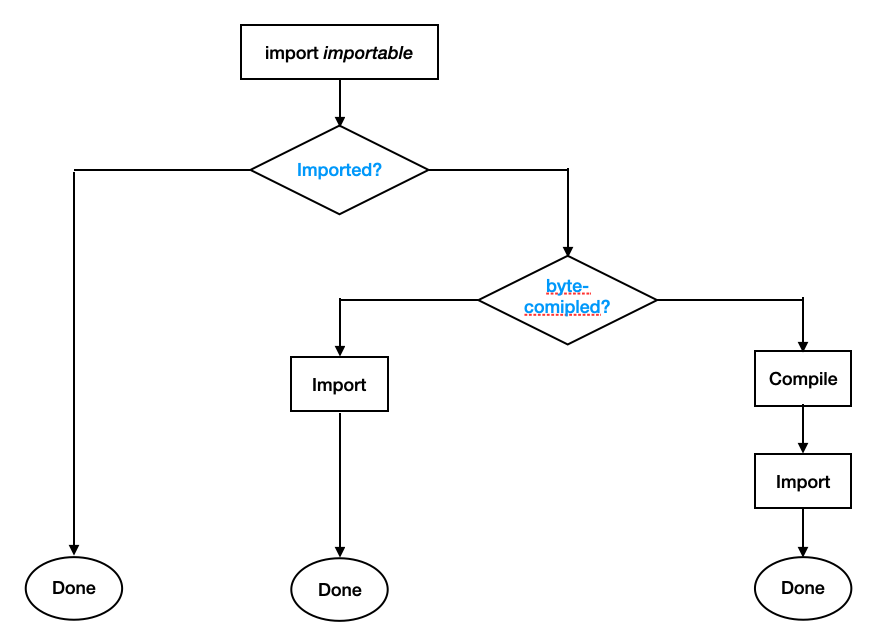
\includegraphics[width=0.8\textwidth]{images/import}
  \caption{Import process}
\end{figure}



\section{Package}
\label{cha:package}

A package is simply a directory that contains a set of modules and a file called \argument{\_\_init\_\_.py}.



In some situations it is convenient to load in all of a \keyword{package}’s modules using a single statement.
To do this we must edit the \keyword{package}’s \argument{\_\_init\_\_.py} file to contain a statement which specifies which modules we want loaded.
This statement must assign a list of module names to the special variable \argument{\_\_all\_\_}.



This syntax can also be applied to a module in which case all the functions, variables, and other object defined in the module (appart from those whose names begin with a leading underscore) will be imported.
If we want to control exactly what is imported, we can define an \argument{\_\_all\_\_} list in the module itself.

\section{Custom module}
\label{sec:custom-module}

You can define your own module.
If you want your module to be available to all your program, there are 3 approaches:
\begin{enumerate}
\item Put the module in the Python distribution's \argument{site-packages} subdirectory.
\item Create a directory for the custom modules and set the \argument{PYTHONPATH} environment variable to this directory
\item Put the module in the local site-packages subdirectory (\argument{/.local/lib/python3.9/site-packages})
\end{enumerate}


The second and third approaches have the advantage of keeping our own code separate from the official installation.


Doctesting is usually done by the following code:
\begin{lstlisting}
if __name__ == '__main__':
    import doctest

    doctest.testmod()
\end{lstlisting}


Whenever a module is imported Python creates a variable for the module called \argument{\_\_name\_\_} and store the modules name in this variable.
A modules name is simply the name of its \argument{.py} file but without the extension.

Whenever a \argument{.py} file is run Python creates a variable for the program called \argument{\_\_name\_\_} and sets it to the string \argument{\_\_main\_\_}.


%%% Local Variables:
%%% mode: latex
%%% TeX-master: "python"
%%% End:


\chapter{Programming techniques}
\label{cha:progr-techn}


\section{Generator}
\label{cha:generator}

Generator provide a means of performing lazy evaluation, which means that they compute only the values that are actually needed.
This can be more efficient than computing a very large list in one go.


There are two ways to create a generator:
\begin{itemize}
\item generator expression
\item the keyword \keyword{yield}
\end{itemize}


\begin{lstlisting}
(expression for item in iterable)
(expression for item in iterable if condition)
\end{lstlisting}

If we need all the items in one go we can pass the generator returned to \funcword{list()} or \funcword{tuple()}.
We can use \funcword{next()} to regrieve the next item from the generator.

\section{Dynamic code execution}
\label{sec:dynam-code-exec}
Dynamic code execution means treating a string as code to evaluate.
There are two built-in functions for dynamic code execution:
\begin{itemize}
\item \funcword{eval()} for expression
\item \funcword{exec()} for code
\end{itemize}

\begin{lstlisting}
x = eval('2 ** 10')
print(x)  # 1024
\end{lstlisting}


\begin{lstlisting}
import math

code = '''
def area_of_sphere(r):
    return 4 * math.pi * r ** 2
'''

context = {}
context['math'] = math
exec(code, context)  # define the function area_of_sphere

\end{lstlisting}


After the \funcword{exec()} call the context dictionary contains a key called \argument{area\_of\_sphere} whose value is the \funcword{area\_of\_sphere()} function.


\begin{lstlisting}
area_of_sphere = context['area_of_sphere']
area = area_of_sphere(5)
print(area)  # 314.1592653589793  

\end{lstlisting}



\section{Decorator}
\label{sec:decorator}

A \keyword{decorator} is a function that takes a function or method as its sole argument and returns a new function or method that incorporates the docorated function or method  with some additional functionality added.

\begin{lstlisting}
@positive_result
def discriminant(a, b, c):
    return b ** 2 - 4 * a * c


def positive_result(function):
    def wrapper(*args, **kwargs):
        result = function(*args, **kwargs)
        assert result >= 0, function.__name__ + "() result isn't >= 0"
        return result

    wrapper.__name__ = function.__name__
    wrapper.__doc__ = function.__doc__
    return wrapper
\end{lstlisting}

Here \funcword{positive\_result} is a decorator.
It define a new local function (here wrapper()) tha calls the original function.
The wrapper finishes by returning the result computed by the wrapped function.
After creating the wrapper, we set its name and docstring to those of the original function.
This helps with introspection, since we want error messages to mention the name of the original function, not the wrapper.
Finally, we return the wrapper function.


We can also use the \argument{functools} module's \funcword{@functools.wraps} decorator to set the function name and docstring to its original ones.
Here's the code:
\begin{lstlisting}
import functools


def positive_result(function):
    @functools.wraps(function)
    def wrapper(*args, **kwargs):
        result = function(*args, **kwargs)
        assert result >= 0, function.__name__ + "() result isn't >=0"
        return result

    return wrapper 
\end{lstlisting}

Here's an example code to create a decorator with parameters.
\begin{lstlisting}
@bounded(0, 100)
def percent(amount, total):
    return (amount / total) * 100

def bounded(minimum, maximum):
    def decorator(function):
        @functools.wraps(function)
        def wrapper(*args, **kwargs):
            result = function(*args, **kwargs)
            if result < minimum:
                return minimum
            elif result > maximum:
                return maximum
            return result

        return wrapper

    return decorator
\end{lstlisting}


Decorators can also be used for logging.
This is a very neat and efficient way for logging.

\section{Function annotation}
\label{sec:function-annotation}

\begin{lstlisting}
def function_name(par1: exp1, par2: exp2, ..., parN: expN) -> rexp:
    suite
\end{lstlisting}

Every colon expression part (: expN) and the return expression part (-> rexp) are optional annotations.

If annotations are present they are added to the function's \argument{\_\_annotations\_\_} dictionary.
If they are not present this dictionary is empty.
The dictionary's keys are the parameter names, and the value are the corresponding expressions.
Annotations have no special significance to Python.
What we can do depends on how we use the \argument{\_\_annotations\_\_} dictionary.
For example to do type checking.

\section{Partial function}
\label{sec:partial-function}

Partial function application is the creation of a function from an existing function and some arguments to produce a new function that does what the original function did, but with some arguments fixed so that callers don’t have to pass them.
Here’s a very simple example:
\begin{lstlisting}
enumerate1 = functools.partial(enumerate, start=1)
for lino, line in enumerate1(lines):
    process_line(lino, line)
\end{lstlisting}



Using partial function application can simplify our code, especially when we want to call the same functions with the same arguments again and again.
For example:

\begin{lstlisting}
reader = functools.partial(open, mode='rt', encoding='utf8')
writer = functools.partial(open, mode='wt', encoding='utf8')
\end{lstlisting}

\begin{lstlisting}
Conv2D_common = functools.partial(Conv2D, kernel_size=(3, 3), activation='relu', padding='same')

h = Conv2D_common(256)(input_layer)
h = Conv2D_common(64)(h)

# The same full code is:
# h = Conv2D(256, (3, 3), activation='relu', padding='same')(input_layer)
# h = Conv2D(64, (3, 3), activation='relu', padding='same')(h)  
\end{lstlisting}

\section{Coroutines}
\label{sec:coroutines}


Coroutines are functions whose processing can be suspended and resumed at specific points.
So, typically, a coroutine will execute up to a certain statement, then suspend execution while waiting for some data.
At this point other parts of the program can continue to execute (usually other coroutines that aren’t suspended).
Once the data is received the coroutine resumes from the point it was suspended, performs processing (presumably based on the data it got), and possibly sending its results to another coroutine.

In Python, a coroutine is a function that takes its input from a \funcword{yield} expression.
It may also send results to a receiver function (which itself must be a coroutine).
Whenever a coroutine reaches a \funcword{yield} expression it suspends waiting for data; and once it receives data, it resumes execution from that point.









%%% Local Variables:
%%% mode: latex
%%% TeX-master: "python"
%%% End:


\chapter{Object-oriented programming}

\section{Costom classes}

\subsection{Attributes and methods}


\begin{tcolorbox}
\begin{verbatim}
class className:
    suite

class className(base_classes):
    suite
\end{verbatim}
\end{tcolorbox}

Just like \verb|def| statements, \verb|class| is a statement, so we can create classes dynamically if we want to.
Class instances are created by calling the class with any necessary arguments.


\begin{lstlisting}
#!/usr/bin/env python3
# Copyright (c) 2021-02

import math


class Point:
    def __init__(self, x=0, y=0):
        """
        A 2D cartesian coordinate
        :param x:
        :param y:
        """
        self.x = x
        self.y = y

    def distance_from_origin(self):
        return math.hypot(self.x, self.y)

    def __eq__(self, other):
        return self.x == other.x and self.y == other.y

    def __repr__(self):
        return f'Point({self.x!r}, {self.y!r})'

    def __str__(self):
        return f'({self.x!r}, {self.y!r})'

\end{lstlisting}


Python automatically supplies the first argument in method calls -- it is an object reference to the object itself.
We must include this argument in the parameter list, and by convention the parameter is called \verb|self|.
All object attributes (data and method attributes) must be qualified by \verb|self|.



To create an object, two steps are necessary:
\begin{enumerate}
\item a raw or uninitialized object must be created (\verb|__new__()|)
\item the object must be initialized, ready for use (\verb|__init__()|)
\end{enumerate}



If we call a method on an object and the object's class does not have an implementation of that method,
Python will automatically go through the object's base classes, and their base classes, and so on, until it finds the method --
and if the method is not found an \verb|AtributeError| exception is raised.



Calling \verb|super().__init__()| is to call the base class's \verb|__init__()| method.
For classes that directly inherit \verb|object| there is no need to do this and we call base class methods only when necessary --
for example, when creating classes that are designed to be subclassed, or
when creating classes that don't directly inherit \verb|object|.



If we want to avoid inappropriate comparisons, we can this:
\begin{lstlisting}
    def __eq__(self, other):
        if not isinstance(other, Point):
            return NotImplemented
        return self.x == other.x and self.y == other.y
\end{lstlisting}
In this case, if \verb|NotImplemented| is returned, Python will then try calling \verb|other.__eq__(self)| to see
whether the \verb|other| type supports the comparion with the \verb|Point| type, and
if there is no such method or if that method alse returns \verb|NotImplemented|, Python will give up and
raise a \verb|TypeError| exception.
Only the following methods may return \verb|NotImplemented|:
\begin{itemize}
\item \verb|__lt__(self, other)|
\item \verb|__le__(self, other)|
\item \verb|__eq__(self, other)|
\item \verb|__ne__(self, other)|
\item \verb|__ge__(self, other)|
\item \verb|__gt__(self, other)|
\end{itemize}




\begin{tcolorbox}
  Poweful \verb|eval()|: (\verb|eval(expression)|)
  \begin{lstlisting}
    p = Shape.Point(3, 9)
    repr(p)                                              # returns: 'Point(3, 9)'
    q = eval(p.__module__ + "." + repr(p))        
    repr(q)                                              # returns: 'Point(3, 9)'
  \end{lstlisting}


  \begin{lstlisting}
    a0 = 0
    a1 = 1
    a2 = 2
    a3 = 3
    
    for i in range(4):
        print(eval(f'a{i} * {i}'))
  \end{lstlisting}

  A more powerful function is \verb|exec()|,
  it can accept python code not only python expression.
  \begin{lstlisting}
    for i in range(3):
        exec(f'a{i} = {i}')
        exec(f'print(a{i})')
    exec('me = "Mike Chyson"')
    print(me)

    exec('''
    def say_hello():
        print('hello')
    ''')
    say_hello()
  \end{lstlisting}

\end{tcolorbox}



\subsection{Inheritance and plymorphism}

\begin{lstlisting}
class Circle(Point):
    def __init__(self, radius, x=0, y=0):
        super().__init__(x, y)
        self.radius = radius

    def edge_distance_from_origin(self):
        return abs(self.distance_from_origin() - self.radius)

    def area(self):
        return math.pi * (self.radius ** 2)

    def circumference(self):
        return 2 * math.pi * self.radius

    def __eq__(self, other):
        return self.radius == other.radius and super().__eq__(other)

    def __repr__(self):
        return f'Circle({self.radius!r}, {self.x!r}, {self.y!r})'

    def __str__(self):
        return repr(self)
\end{lstlisting}



\subsection{Using properties to control attribute access}

\begin{tcolorbox}
A property is an item of object data that is accessed like an instance variable
but where the accesses are handled methods behind the scenes.
\end{tcolorbox}


\begin{lstlisting}
class Circle(Point):
    def __init__(self, radius, x=0, y=0):
        super().__init__(x, y)
        self.radius = radius

    @property
    def edge_distance_from_origin(self):
        return abs(self.distance_from_origin - self.radius)

    @property
    def area(self):
        return math.pi * (self.radius ** 2)

    @property
    def circumference(self):
        return 2 * math.pi * self.radius

    @roperty
    def radius(self):
        return self.__radius

    @property.setter
    def radius(self, radius):
        assert radius > 0, 'radius must be nonzero and non-negative'
        self.__radius = radius  
\end{lstlisting}

\begin{tcolorbox}
  A decorator is a function that takes a function or method as its argument and returns a ``decorated'' version,
  that is, a version of the function or method that is modified in some way.
  A decorator is indicated by preceding its name with an at symbol (@). 
\end{tcolorbox}



The \verb|property()| decorator function is built-in and takes up to four arguments:
\begin{itemize}
\item a getter function
\item a setter function 
\item a deleter function
\item a docstring
\end{itemize}

The effect of using \verb|@property| is the same as calling the \verb|property()| function with just one argument, the getter function.
We could have created the area property like this:
\begin{lstlisting}
  def area(self):
      return math.pi * (self.radius ** 2)
  area = property(area)
\end{lstlisting}
We rarely use this syntax, since using a decorator is shorter and clearer.





To turn an attribute into a readable/writable property we must create a private attribute where the data is actually held and supply getter and setter methods.
\begin{lstlisting}
    @property
    def radius(self):
        return self.__radius

    @property.setter
    def radius(self, radius):
        assert radius > 0, 'radius must be nonzero and non-negative'
        self.__radius = radius   
\end{lstlisting}


Every property that is created has a \verb|getter|, \verb|setter|, and \verb|deleter| attribute,
so once the radius property is created using \verb|@property|, the \verb|radius.getter|, \verb|radius.setter|, and
\verb|radius.deleter| attributes become available.
The \verb|radius.getter| is set to the getter method by the \verb|@property| decorator.
The other two are set up by Python so that they do nothing (so the attribute cannot be written to or deleted),
unless they are used as decorators, in which case they in effect replace themselves with the method they are used to decorate.


The \verb|Circle|'s initializer, \verb|Circle.__init__()|, includes the statement \verb|self.radius = radius|;
this will call the \verb|radius| properity's setter.





\chapter{Processes and threading}
\label{cha:processes-threading}

There are two main approaches to spreading the workload:
\begin{itemize}
\item multiple processes
\item multiple threads
\end{itemize}



\begin{table}[htb!]
  \centering
  \begin{tabular}{p{0.2\columnwidth}p{0.35\columnwidth}p{0.35\columnwidth}}
    \toprule{}
    & \head{advantage} & \head{disadvantage} \\
    \midrule
    multiple processes & each process runs independently & communication and data sharing can be inconvenient \\
    multiple threads & can communicate simply by data sharing & more complex than single-threaded program\\
    \bottomrule
  \end{tabular}
  \caption{multiple processes and multiple threads}
\end{table}




%%% Local Variables:
%%% mode: latex
%%% TeX-master: "python"
%%% End:


% Pages are numbered with Arabic numbers.
% Chapters generate a table of contents entry but don't get a number.
\backmatter{}
\cleardoublepage{}
\phantomsection{}
\nocite{*}
\bibliographystyle{plain}       % % plain, unsrt, alpha, abbrv
\bibliography{tex}

\cleardoublepage{}
% just setting an anchor like \hypertarget{}{}
% fix the problem that anchor point to the previous section
\phantomsection{}                 
\printindex{}
\end{document}





%%% Local Variables:
%%% mode: latex
%%% TeX-master: t
%%% End:
